\documentclass[tikz, border=10pt]{standalone}
\usepackage{tikz}
\usepackage{amsmath}
\usetikzlibrary{calc, arrows.meta}

\begin{document}
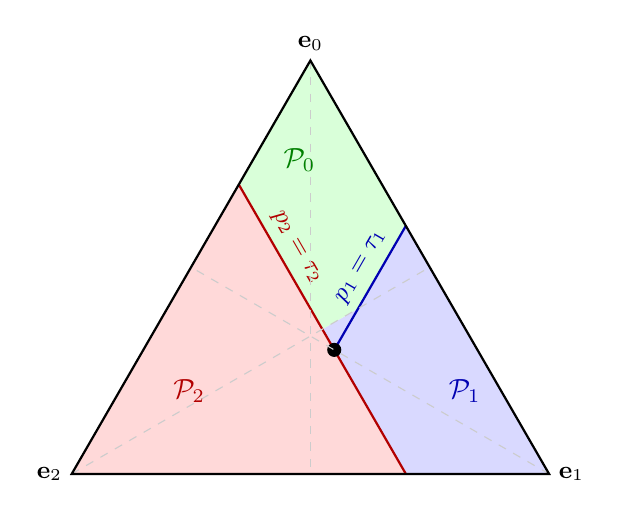
\begin{tikzpicture}[font=\sffamily, scale=0.7]

    % Vertices
    \coordinate (T) at (0, 5);          % Class 0 (p_0=1)
    \coordinate (R) at (4.33, -2.5);    % Class 1 (p_1=1)
    \coordinate (L) at (-4.33, -2.5);   % Class 2 (p_2=1)

    % Threshold contour endpoints:
    % p_2 = 0.30 line:
    %   Top-Left edge (p_1=0): (0.70, 0, 0.30) -> (-1.299, 2.75)
    %   Right-Left edge (p_0=0): (0, 0.70, 0.30) -> (1.732, -2.5)
    \coordinate (T2a) at (-1.299, 2.75);
    \coordinate (T2b) at (1.732, -2.5);

    % p_1 = 0.40 line:
    %   Top-Right edge (p_2=0): (0.60, 0.40, 0) -> (1.732, 2.0)
    %   Right-Left edge (p_0=0): (0, 0.40, 0.60) -> (-0.866, -2.5)
    \coordinate (T1a) at (1.732, 2.0);
    \coordinate (T1b) at (-0.866, -2.5);

    % Intersection of p_2=0.30 and p_1=0.40: (0.30, 0.40, 0.30) -> (0.433, -0.25)
    \coordinate (Corner) at (0.433, -0.25);

    % ===== Region fills =====

    % Argmax median (p_0=p_1) intersects the fallback region at two points:
    %   MedOnBlue: on p_1=0.40 line at (0.35, 0.35, 0.30) -> (0.2165, 0.125)
    %     Wait: (p0=0.35, p1=0.35, p2=0.30) -> x=4.33*(0.35-0.30)=0.2165, y=7.5*0.35-2.5=0.125
    %   MedOnP1: on p_1=0.40 line at (0.30, 0.40, 0.30)... that's Corner itself
    %     Actually: median L-MidTR intersects p_1=0.40 at (0.30, 0.40, 0.30)
    %     but Corner=(0.30, 0.40, 0.30) IS the intersection of p1=0.40 and p2=0.30.
    %     The median hits p_1=0.40 at (p0, 0.40, p2) where p0=p1=0.40... wait no.
    %     p0=p1 and p1=0.40 means p0=0.40, p2=0.20.
    %     -> x=4.33*(0.40-0.20)=0.866, y=7.5*0.40-2.5=0.5
    \coordinate (MedOnRed) at (0.2165, 0.125);  % p0=p1 meets p2=0.30
    \coordinate (MedOnBlue) at (0.866, 0.5);     % p0=p1 meets p1=0.40

    % Class 2 (red, priority 1): p_2 >= 0.30
    \fill[red!15] (T2a) -- (T2b) -- (L) -- cycle;

    % Class 1 (blue, priority 2): p_2 < 0.30 AND p_1 >= 0.40
    \fill[blue!15] (T1a) -- (Corner) -- (T2b) -- (R) -- cycle;

    % Class 1 (blue, fallback argmax): p_2 < 0.30 AND p_1 < 0.40 AND p_1 > p_0
    \fill[blue!15] (MedOnBlue) -- (Corner) -- (MedOnRed) -- cycle;

    % Class 0 (green, fallback argmax): p_2 < 0.30 AND p_1 < 0.40 AND p_0 > p_1
    \fill[green!15] (T) -- (T1a) -- (MedOnBlue) -- (MedOnRed) -- (T2a) -- cycle;

    % ===== Threshold contour lines =====

    % p_2 = tau_2 line (separates class 2 from rest)
    \draw[thick, red!70!black] (T2a) -- (T2b)
        node[sloped, above, pos=0.25, font=\small, red!70!black] {$p_2 = \tau_2$};

    % p_1 = tau_1 line (separates class 1 from class 0, within p_2 < tau_2)
    \draw[thick, blue!70!black] (T1a) -- (Corner)
        node[sloped, above, pos=0.4, font=\small, blue!70!black] {$p_1 = \tau_1$};

    % Corner marker (the "step" — key visual)
    \node[circle, fill=black, inner sep=1.8pt] at (Corner) {};

    % ===== Argmax boundaries (dashed, for comparison) =====
    \coordinate (MidTR) at (2.165, 1.25);
    \coordinate (MidTL) at (-2.165, 1.25);
    \coordinate (MidRL) at (0, -2.5);
    \draw[dashed, gray!40, thin] (L) -- (MidTR);
    \draw[dashed, gray!40, thin] (R) -- (MidTL);
    \draw[dashed, gray!40, thin] (T) -- (MidRL);

    % ===== Triangle frame =====
    \draw[thick] (T) -- (R) -- (L) -- cycle;

    % ===== Labels =====

    % Vertex labels
    \node[above, font=\small] at (T) {$\mathbf{e}_0$};
    \node[right, font=\small] at (R) {$\mathbf{e}_1$};
    \node[left, font=\small] at (L) {$\mathbf{e}_2$};

    % Region labels
    \node[green!50!black, font=\normalsize\bfseries] at (-0.2, 3.2) {$\mathcal{P}_0$};
    \node[blue!70!black, font=\normalsize\bfseries] at (2.8, -1.0) {$\mathcal{P}_1$};
    \node[red!70!black, font=\normalsize\bfseries] at (-2.2, -1.0) {$\mathcal{P}_2$};

\end{tikzpicture}
\end{document}
